%%% Math 340
%%% Homework 5

\documentclass{article}

\usepackage[utf8]{inputenc}
\usepackage[top=1.5in,left=1in,right=1in,bottom=1.5in,headheight=1in]{geometry}
\usepackage{fancyhdr}
\usepackage{lastpage}
\usepackage{amsmath,amsthm}
\usepackage{enumerate}
\usepackage{listings}
\usepackage{multicol}
\usepackage{graphicx}

\newtheoremstyle{problem}
{\topsep}% Above space
{\topsep}% Below space
{}%         Body font
{}%         Indent amount (empty = no indent, \parindent = para indent)
{\bfseries}% Thm head font
{\vspace{5pt}}%        Punctuation after thm head
{\newline}%     Space after thm head (\newline = linebreak)
{\thmname{#1}\thmnote{ #3}}%         Thm head spec

\theoremstyle{problem}
\newtheorem{prob}{Problem}
\theoremstyle{remark}
\newtheorem*{answer}{Answer}

%%% Heading -- No need to edit %%%
\pagestyle{fancy}
\rhead{
  Stefan Eng \\ 
  William Watkins \\ 
  Math 340 \\ 
  10/7/13
}
\lhead{
  Chapter 3\\
  103, 107, 115, 119
}
\cfoot{Page\ \thepage\ of\ \pageref{LastPage}}
%%% 

% No indent for whole page
\setlength\parindent{0pt}

\begin{document}

%%% Make the title %%%
\begin{center}
  \textsc{\Large Introduction to Probability}\\[.3cm]
  \textsc{\Large Homework 6}
\end{center}
%%% End title %%%

%%% Start Assignment Here %%%
\begin{prob}[103]
A warehouse contains ten printing machines, four of which are defective. A company selects five of the machines at random, thinking all are in working condition. What is the probability that all five of the machines are non defective.
\end{prob}
\begin{answer}
$$
\frac{\displaystyle {6 \choose 5}}{\displaystyle {10 \choose 5}} = \frac{6}{252} = \frac{1}{42}
$$
\end{answer}
% 

\begin{prob}[107]
A group of six software packages available to solve a linear programming problem has been ranked from 1 to 6 (best to worst). An engineering firm, unaware of the rankings, randomly selected and then purchased two of the packages. Let $Y$ denote the number of packages purchased by the firm that are ranked 3, 4, 5, or 6. Give the probability distribution for $Y$.
\end{prob}
\begin{answer}
  We have a hypergeometric distribution with parameters $N = 6$, $n = 2$, and $r = 4$.
\begin{align*}
y = 0: \frac{\displaystyle {2 \choose 2}}{ \displaystyle {6 \choose 2}} = \frac{1}{15}&&
y = 1: \frac{\displaystyle {2 \choose 1} {4 \choose 1}}{ \displaystyle {6 \choose 2}} = \frac{8}{15}&&
y = 2: \frac{\displaystyle {4 \choose 2}}{ \displaystyle {6 \choose 2}} = \frac{6}{15}&&
\end{align*}
\end{answer}
% 

\begin{prob}[115]
Suppose that a radio contains six transistors, two of which are defective. Three transistors are selected at random, removed from the radio, and inspected. Let $Y$ equal the number of defectives observed, where $Y = 0, 1,$ or $2$. Find the probability distribution of $Y$. Express your results graphically as a probability histogram.
\end{prob}
\begin{multicols}{2}
\lstinputlisting[language=R,showstringspaces=false]{prob_hist_115.R}
\vfill
\columnbreak
\begin{center}
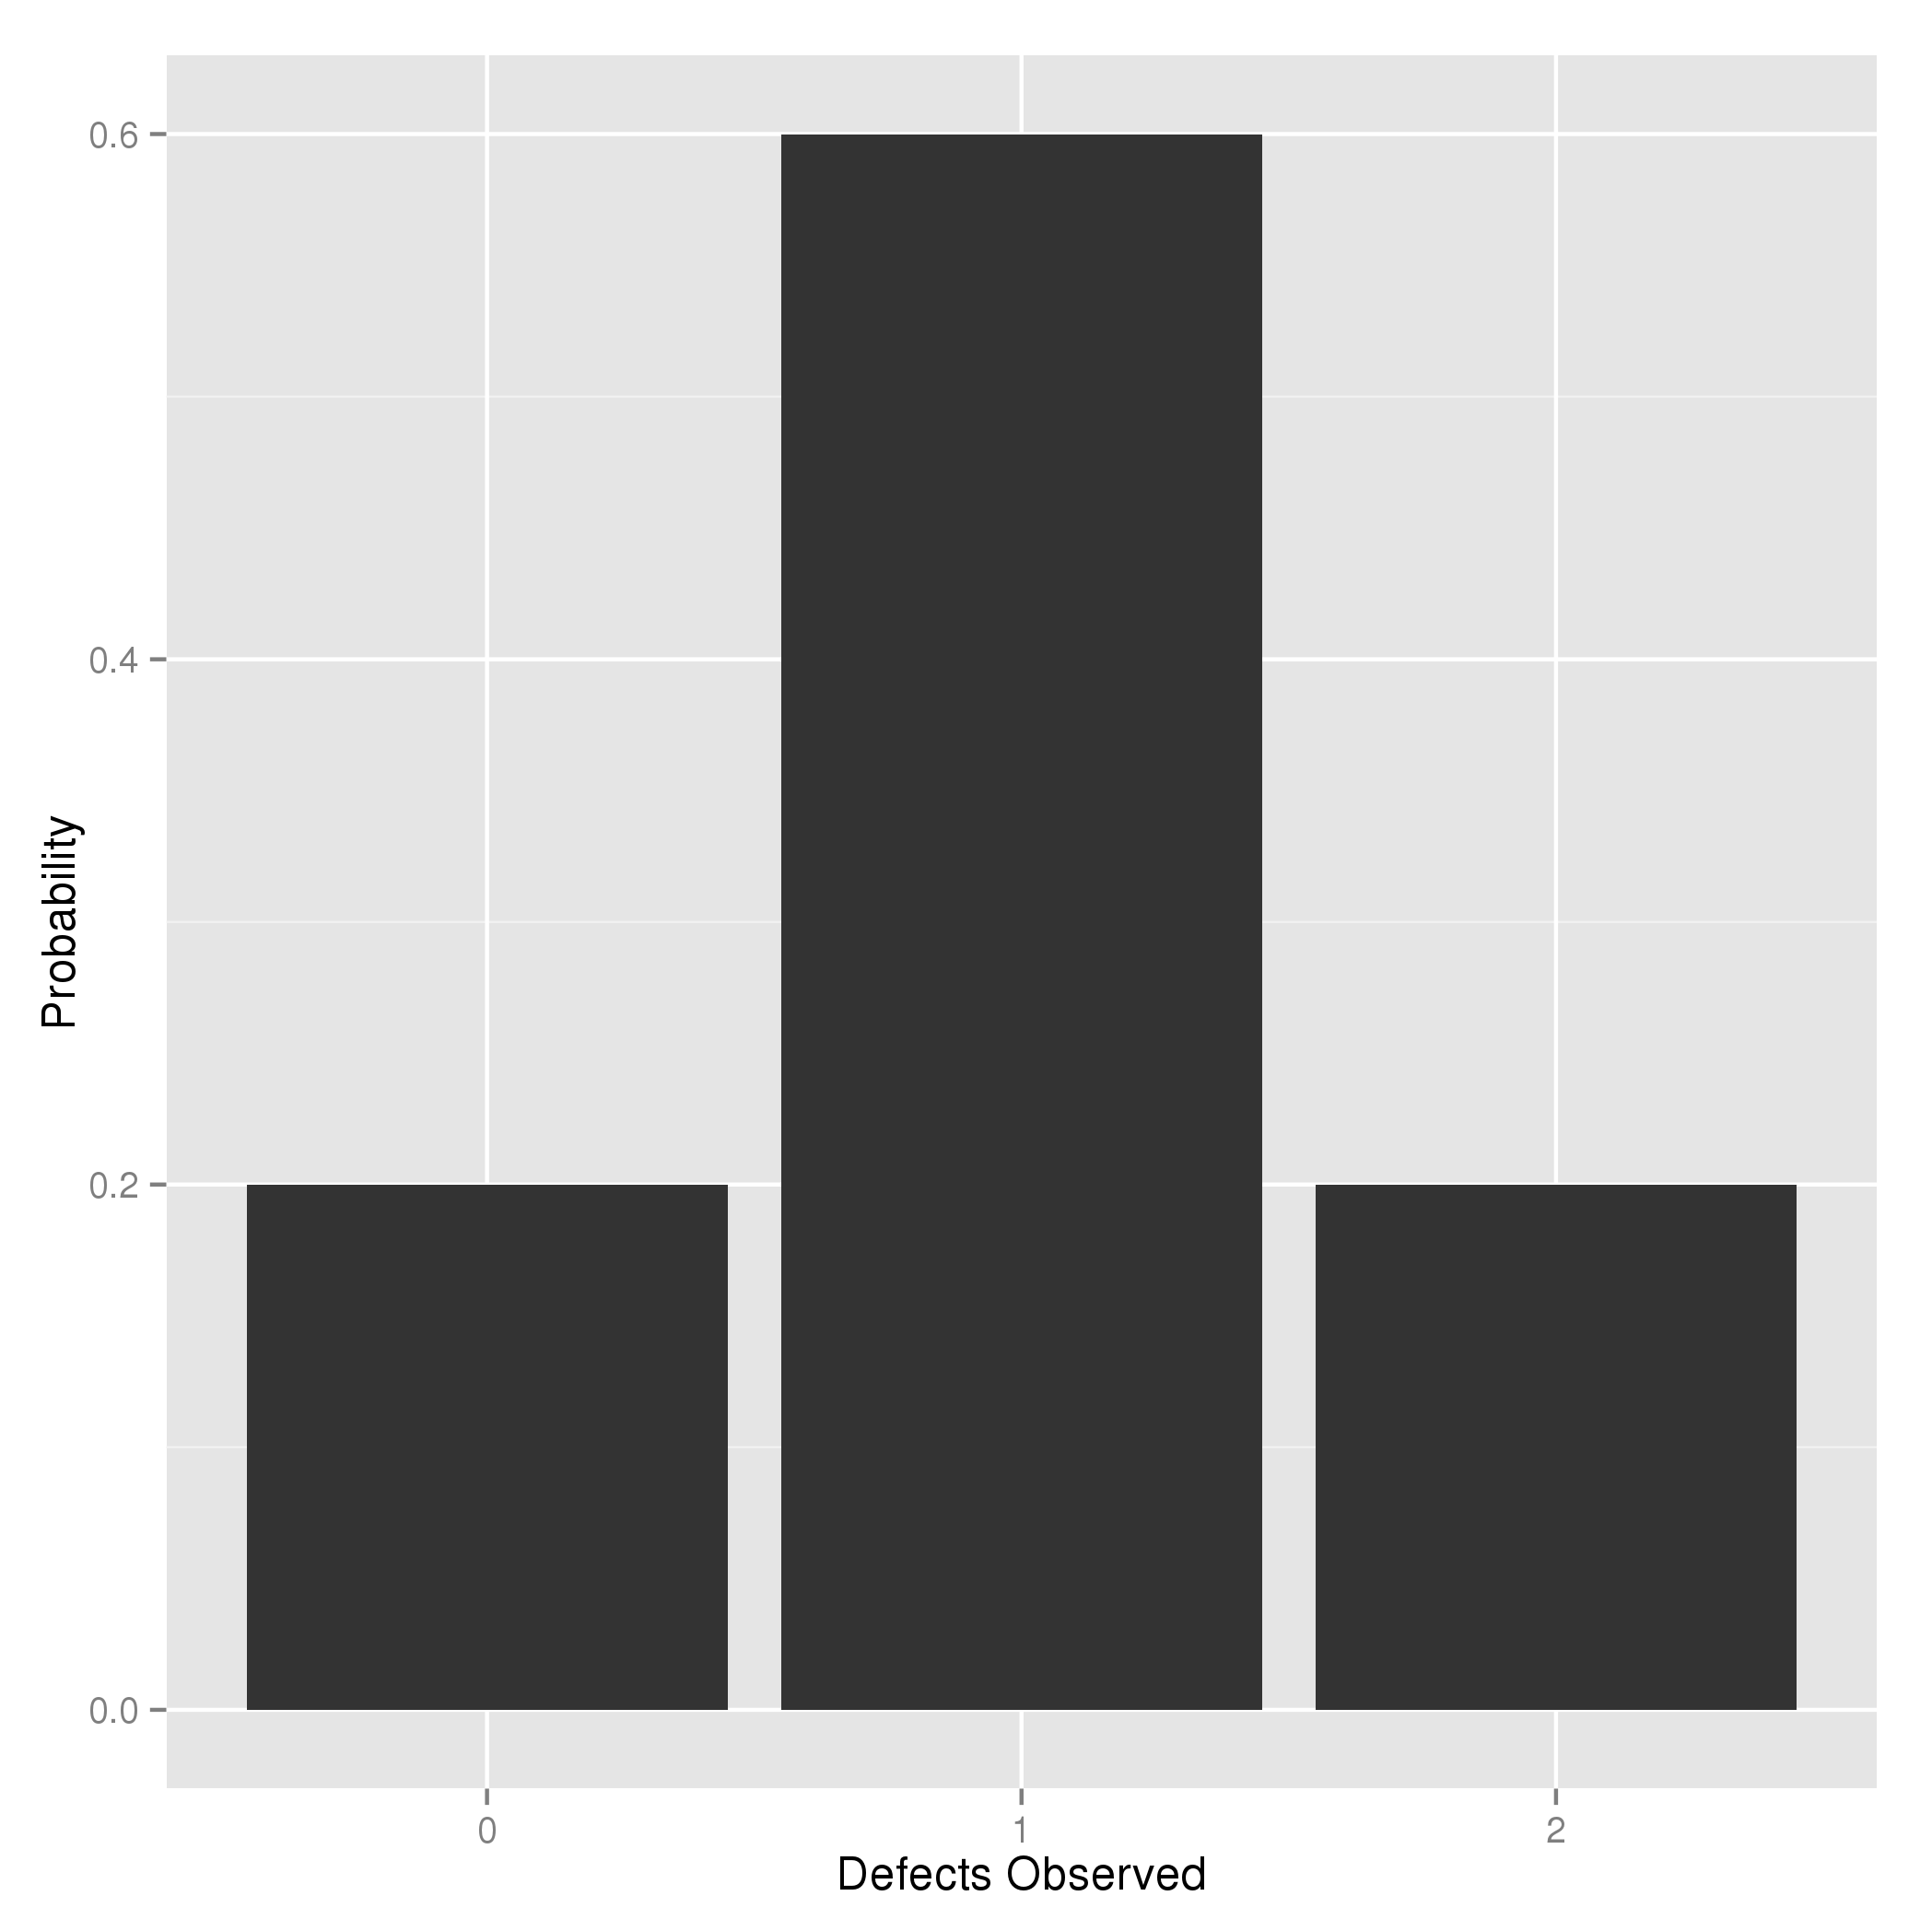
\includegraphics[scale=.35]{problem115.png}
\end{center}
\end{multicols}
% 


\begin{prob}[119]
Cards are dealt at random and without replacement from a standard 52 card deck. What is the probability that the second king is dealt on the fifth card.
\end{prob}
\begin{answer}
Let $A$ be the even that the first four cards contain one king and three non-kings. Let $B$ be the even that the fifth card is the second king. The probability of $A$ is a straight hypergeometric probability of drawing one of the four kings and three of the remaining non-kings.
$$
P(A) = \frac{\displaystyle {4 \choose 1} {48 \choose 3}}{\displaystyle {52 \choose 4}}
$$ 
Now given that the first four cards have been drawn and the one is a king and the other three are non-kings, the porbability tat the fifth card is a king is given below:
$$
P(B|A) = \frac{3}{48}
$$
since there  are three kings left in the eck of 48 cards. Now we have:
$$
P(B) = P(B|A)P(A) = \frac{3}{48} \frac{\displaystyle {4 \choose 1} {48 \choose 3}}{\displaystyle {52 \choose 4}} = 0.0159719
$$
\end{answer}
% 

\end{document}

%%% End assignment %%%
